%
% file: localoperator.tex
% author: Victor Brena
% description: Briefly describes properties of the local operator.
%

\chapter{Appendix D}\label{app:app04}
Psuedo code for distance metrics
\begin{algorithm}
    Generate line vector segments based on waypoints: line_vecs
    Get a vector from the start of each line segment(line_vecs) vector to each point: line_to_recorded_vecs
    dot_prod = dot($\frac{line\_to\_recorded\_vecsline\_vecs}{|line\_vecs|}$)
    projections = min($\frac{line\_vecs}{|line\_vecs|}$, max(0, dot_prod))
    norm_line_vecs = $\frac{line\_vecs}{|line\_vecs|}$
    distances = length(line_to_recorded_vecs - projections*norm_line_vecs)
    get_min_distance_for_each_point(distances)

\end{algorithm}

\chapter{Appendix E}\label{ch:appendix-e}
\begin{figure}[h!]
    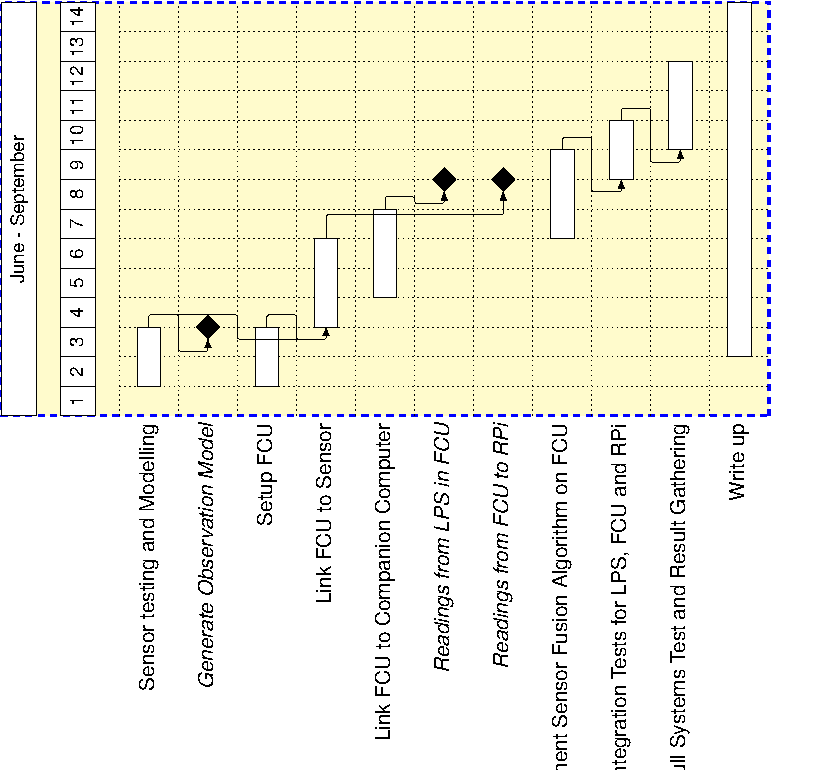
\includepdf[scale=0.4, angle=-90]{Gantt_Charts_with_the_pgfgantt_Package.pdf}
\end{figure}

\chapter{Appendix F}\label{ch:appendix-f}
\newpage
\section{Ethical Review Checklist}
\begin{figure}[h!]
    
\includepdf[scale=0.5, page=1]{Ethical_Review_Checklist.pdf}
\end{figure}
\newpage
\section{Ethical Review Checklist (cont'd)}
\begin{figure}[h!]
    
\includepdf[scale=0.5, page=2]{Ethical_Review_Checklist.pdf}
\end{figure}